

\section{Introduction}

%From Wikipedia, the free encyclopedia.
%
%In probability theory and statistics, a Gaussian process is a particular kind of statistical model where observations occur in a continuous domain, \eg time or space. In a Gaussian process, every point in some continuous input space is associated with a normally distributed random variable. Moreover, every finite collection of those random variables has a multivariate normal distribution, i.e. every finite linear combination of them is normally distributed. The distribution of a Gaussian process is the joint distribution of all those (infinitely many) random variables, and as such, it is a distribution over functions with a continuous domain, e.g. time or space. 
%
%
%Viewed as a machine learning algorithm, a Gaussian process uses lazy learning and a measure of the similarity between points (the kernel function) to predict the value for an unseen point from training data. The prediction is not just an estimate for that point, but also has uncertainty information it is a one-dimensional Gaussian distribution (which is the marginal distribution at that point).
%
%For some kernel functions, matrix algebra can be used to calculate the predictions using the technique of Kriging. When a parameterized kernel is used, optimization software is typically used to fit a Gaussian process model.
%
%The concept of Gaussian processes is named after Carl Friedrich Gauss because it is based on the notion of the Gaussian distribution (normal distribution). Gaussian processes can be seen as an infinite-dimensional generalization of multivariate normal distributions.
%
%Gaussian processes are useful in statistical modeling, benefiting from properties inherited from the normal. For example, if a random process is modeled as a Gaussian process, the distributions of various derived quantities can be obtained explicitly. Such quantities include the average value of the process over a range of times and the error in estimating the average using sample values at a small set of times.


Consider a regression problem with observations $y_i = f(t_i)+\epsilon_i$, $i=1,\ldots,n$, containing i.i.d normal noises $\epsilon_i\sim N(0,\sigma^2)$, a classic nonparametric or semi-parametric regression is a function that minimizes the following penalized least square function 
\begin{equation}
\frac{1}{n}\sum_{i=1}^{n}\left( y_i-f(t_i) \right)^2 + \lambda J(f),
\end{equation}
where $J(f)$ is a quadratic functional measuring the roughness of $f$ \cite{kim2004smoothing}. The first term is the lack of fit of $f$ to the data. In the second term, generally, $\lambda$ is a fixed smoothing parameter controlling the trade-off between over-fitting and bias. For instance, cubic smoothing spline provides a powerful tool to estimate the above nonparametric functions with penalty term $J(f) = \int f''^2dt$ \cite{hastie1990generalized}. 



\subsection{Spline}

In interpolation and curve fitting, piecewise linear approximation may not have the practical significance of cubic spline, or even higher order, approximation. These "broken lines" are neither very smooth nor very efficient approximation. Researchers can go to piecewise polynomial approximation with higher order pieces \cite{de1978practical}, which is called spline method. A spline is a numeric function that is piecewise-defined by polynomial functions, and which possesses a high degree of smoothness at the places where the polynomial pieces connect (known as knots) \cite{judd1998numerical}\cite{chen2009feedback}. Suppose we are given observed data $t_1,t_2, \ldots, t_n$ on interval $[0,1]$, satisfying $0\leq t_1< t_2 < \cdots <t_n \leq 1$. A piecewise polynomial function $f(t)$ can be obtained by dividing the interval into contiguous intervals $(t_1,t_2),\ldots,(t_{n-1},t_n)$ and represented by a separate polynomial in each interval. For any continuous $f\in \mathbb{C}^{(m)}[0,1]$, it can be represented in a linear combination of basis functions $h_m(t)$, just as every vector in a vector space can be represented as a linear combination of basis vectors. So we have
\begin{equation}\label{fbasis}
f(t) =\sum_{m=1}^{M}\beta_mh_m(t),
\end{equation}
where $\beta_m$ are coefficients \cite{ellis2009}. 

Suppose we were attempt to fit a model of $f(t)$ by least squares without any restrictions, the best fitting $\hat{f}(t)$ would go through every given data to reduce sum of squares to zero. Most of the time, the results are unsatisfactory as explanations of the given data. The roughness penalty approach is introduced to quantify the notion of a rapidly fluctuating curve and then to pose the estimation problem in a way that makes explicit the necessary compromise between varying rapidly fluctuation and slowly trend in curve estimation \cite{green1993nonparametric}. By adding a penalty term $\int_{0}^{1}(f^{(m)}(t))^2dt$, the curve estimate $\hat{f}(t)$ exists and is unique over all spline functions $f(t)$ with $m-1$ continuous derivatives fitting observed data in the space $\mathbb{C}^{(m)}[0,1]$, and it can be found by minimizing the following penalized mean residual sum  squares
\begin{equation}\label{GaussianProcessMSEFunction}
\text{MSE}(f,\lambda)=\frac{1}{n}\sum_{i=1}^n(f(t_i)-y_i)^2+\lambda \int_{0}^{1}(f^{(m)}(t))^2dt,
\end{equation}
where $\lambda$ is a fixed smoothing parameter, $(t_i,y_i)$, $i=1, \ldots, n$ are observed data and $0 \leq t_1< t_2 < \cdots <t_n \leq 1$. In equation (\ref{GaussianProcessMSEFunction}),  the smoothing parameter $\lambda$ controls the trade-off between over-fitting and bias. Smoothing spline provides a powerful tool to estimate nonparametric functions \cite{hastie1990generalized}. 

\subsection{Gaussian Process Regression}

A Gaussian Process is a collection of random variables, any finite number of which have a joint Gaussian distribution \cite{b_gpml}. It is fully defined by its mean $m(t)$ and covariance $K(s,t)$ functions as
\begin{align}
m(t)&=\E [f(t)] \\
K(s,t)&=\E \lbrack (f(s)-m(s)) (f(t)-m(t))\rbrack,
\end{align}
where $s$ and $t$ are two variables, and a function $f$ distributed as such is denoted in form of
\begin{equation}
f \sim GP(m(t),K(s,t)).
\end{equation}
Usually the mean function is assumed to be zero everywhere. 

Given a set of input variables $\mathbf{T}$ for function $f(t)$ and the output $\mathbf{y}=f(\mathbf{T})+\varepsilon$ with independent identically distributed Gaussian noise $\varepsilon$ with variance $\sigma_n^2$,  we can use the above definition to predict the value of the function $f_*=f(t_*)$ at a particular input $t_*$. As the noisy observations becoming
\begin{align}\label{GaussianProcessCovDef}
\Cov (y_p,y_q) = K(t_p,t_q)+\sigma_n^2 \delta_{pq}
\end{align}
where $\delta_{pq}$ is a Kronecker delta which is one iff $p=q$ and zero otherwise, the joint distribution of the observed outputs $\mathbf{y}$ and the estimated output $f_*$ according to prior is
\begin{equation}
\begin{bmatrix}
\mathbf{y}\\
f_*
\end{bmatrix} \sim N \left(  
0,  \begin{bmatrix}
K(\mathbf{T},\mathbf{T}) +\sigma_n^2I& K(\mathbf{T},t_*) \\
K(t_*,\mathbf{T}) & K(t_*,t_*)
\end{bmatrix} 
\right).
\end{equation}
The posterior distribution over the predicted value is obtained by conditioning on the observed data
\begin{equation}
f_* \mid  \mathbf{y},\mathbf{T},t_* \sim N(\bar{f_*},\Cov (f_*))
\end{equation}
where 
\begin{align}
\bar{f_*}&=\E [f_* \mid  \mathbf{y},\mathbf{T},t_* ]=K(t_*,\mathbf{T})[K(\mathbf{T},\mathbf{T})+\sigma_n^2I]^{-1}\mathbf{y},\\
\Cov(f_*)&=K(t_*,t_*)-K(t_*,\mathbf{T})[K(\mathbf{T},\mathbf{T})+\sigma_n^2I]^{-1}K(\mathbf{T},t_*).
\end{align}


\subsection{Reproducing Kernel Hilbert Space}



\subsection{The Smoothing Spline as Bayes Estimates}
It is possible to interpret the smoothing spline regression estimator as a Bayesian estimate when the mean function $r( .)$ is given an improper prior distribution. \cite{berlinet2011reproducing}
\cite{wahba1990spline}


Consider the model
\begin{equation}
y_i=f(t_i)+\varepsilon_i, 
\end{equation}
where $i=1, \ldots, n$, $\varepsilon_i$ are i.i.d. Gaussian distributed noise with variance $\sigma^2$. Assume $f\in \mathbb{H}^{(m)}[0,1]$, where
\begin{equation}
\mathbb{H}^{(m)}[0,1]=\{f:f^{(\nu)} \mbox{absolutely continuous}, \nu=0,\ldots,m-1, \int_{0}^{1} (f^{(m)}(t)^2dt<\infty \}.
\end{equation}
A smoothing spline $\hat{f}_\lambda$ is the minimizer of objective function (\ref{GaussianProcessMSEFunction}) \cite{wang1998smoothing}. Equipped with an appropriate inner product
\begin{equation}
\langle f,g\rangle=\sum_{\nu=0}^{m-1}f^{(\nu)}(0)g^{(\nu)}(0)+\int_{0}^{1}f^{(m)}g^{(m)}dt,
\end{equation}
the space $\mathbb{H}^{(m)}[0,1]$ becomes a reproducing kernel Hilbert space.

Let $\phi_\nu (t)=\frac{t^{\nu-1}}{(\nu-1)!}$ where $\nu=1, \ldots, m$ and $R_1(s,t)=\int_0^1\frac{ (s-u)_+^{m-1}}{(m-1)!} \frac{ (t-u)_+^{m-1}}{(m-1)!} du$. Denote $S=\{\phi_\nu (t_i) \}_{n\times m}$ where $i=1, \ldots, n$, $\nu=1, \ldots, m$ and $Q=\{ R_1(t_i,t_j)\}_{n\times n}$ where $i=1, \ldots, n$, $j=1, \ldots, n$. \cite{kimeldorf1971some} and \cite{kimeldorf1970correspondence}  proved that $\hat{f}_\lambda$ has the form
\begin{equation}
\hat{f}(t)=\sum_{\nu=1}^m d_\nu \phi_\nu(t)+\sum_{i=1}^n c_iR_1(t,t_i).
\end{equation}
By denoting $M=Q+n\lambda I$, \cite{gu2013smoothing} found that the coefficients will be given by
\begin{align}
\mathbf{c}&=(M^{-1}-M^{-1}S(S^\top M^{-1}S)^{-1}S^\top M^{-1})\mathbf{Y},\\
\mathbf{d}&=(S^\top M^{-1}S)^{-1}S^\top M^{-1}\mathbf{Y}.
\end{align}



\section{Tractor Spline}


\section{Reproducing Kernel Hilbert Space on $\mathcal{C}_{p.w.}^{2}[0,1]$}
The minimizer $f(x)$ of
\begin{equation}\label{maineq}
\frac{1}{n}\sum_{i=1}^{n}(Y_i-f(x_i))^2+\frac{\gamma}{n}\sum_{i=1}^{n}(v_i-f'(x_i))^2+\lambda \int_{0}^{1}f''^2dx
\end{equation}
in the space $\mathcal{C}_{p.w.}^{2}[0,1]=\{f:f,f' \mbox{ are continuous and } f'' \mbox{ is piecewise continuous on } [0,1] \}$ is a tractor spline. Equipped with an appropriate inner product
\begin{equation}
(f,g)=f(0) g(0)+f'(0) g'(0)+\int_{0}^{1}f''g''dx,
\end{equation}
the space $\mathcal{C}_{p.w.}^{2}[0,1]$ is made a reproducing kernel Hilbert space. In fact, the representer $R_x(\cdot)$ is 
\begin{equation}\label{kerneleq}
R_x(y)=1+xy+\int_{0}^{1} (x-u)_+(y-u)_+du.
\end{equation}
It can be seen that $R_x(0)=1, R'_x(0)=x$, and $R''_x(y)=(x-y)_+$.

The two terms of the reproducing kernel $R(x,y)=R_x(y)=R_0(x,y)+R_1(x,y)$, where
\begin{align}
R_0(x,y)&=1+xy \\
R_1(x,y)&=\int_{0}^{1} (x-u)_+(y-u)_+du
\end{align}
are both non-negative definite themselves.

\begin{theorem}
If the reproducing kernel $R$ of a space $\mathcal{H}$ on domain $X$ can be decomposed into $R = R_0+R_1$, where $R_0$ and $R_1$ are both non-negative definite, $R_0(x,\cdot), R_1(x,\cdot) \in \mathcal{H}$, $\forall x \in X$, and $(R_0(x, ·),R_1(y, ·)) = 0$, $\forall x, y \in X$, then the spaces $\mathcal{H}_0$ and $\mathcal{H}_1$ corresponding respectively to $R_0$ and $R_1$ form a tensor sum decomposition of $\mathcal{H}$. Conversely, if $R_0$ and $R_1$ are both non-negative definite and $\mathcal{H}_0 \cap \mathcal{H}_1 = \{ 0 \}$, then $\mathcal{H} = \mathcal{H}_0 \bigoplus \mathcal{H}_1$ has a reproducing kernel $R = R_0 + R_1$.
\end{theorem}

According to Theorem 1, $R_0$ can correspond the space of polynomials $\mathcal{H}_0=\{f:f''=0\}$ with an inner product $(f,g)_0= f(0)g(0)+f'(0)g'(0)$, and $R_1$ corresponds the orthogonal complement of $\mathcal{H}_0$
\begin{equation*}
\mathcal{H}_1=\{f:f(0)=0, f'(0)=0, \int_{0}^{1}f''^2dx<\infty\}
\end{equation*}
with inner product $(f,g)_1=\int_{0}^{1}f''g''dx$. Thus, $\mathcal{H}_0$ and $\mathcal{H}_1$ are two subspaces of the $\mathcal{C}_{p.w.}^{2}[0,1]$, and the reproducing kernel is $R_x(\cdot) = R_0(x,\cdot)+R_1(x,\cdot)$.

Define a new notation $\dot{R}(x,y)=\frac{\partial R}{\partial x}(x,y)=\frac{\partial R_0}{\partial x}(x,y)+\frac{\partial R_1}{\partial x}(x,y)=y+\int_0^x(y-u)_+du$. Obviously $\dot{R}_x(y) \in \mathcal{C}_{p.w.}^{2}[0,1]$. Additionally, we have $\dot{R}_x(0)=0, \dot{R}'_x(0)=\frac{\partial \dot{R}_x}{\partial y}(0)=1$, and $ \dot{R}''_x(y)=\begin{cases}
0 & x\leq y \\ 1 & x>y \end{cases}$. Then, for any $f\in \mathcal{C}_{p.w.}^{2}[0,1]$, it gives us 
\begin{align*}
(\dot{R}_x,f) &=\dot{R}_x(0)f(0)+\dot{R}'_x(0)f'(0)+\int_0^1\dot{R}''_x f''	 du=f'(0)+\int_0^y f''du=f'(y).
\end{align*}
It can be seen that the first term $\dot{R}_0=y\in \mathcal{H}_0$, and the space spanned by the second term  $\dot{R}_1=\int_0^x(y-u)_+du$, denoted as $\mathcal{\dot{H}}$, is not in $\mathcal{H}_1$, but $\mathcal{\dot{H}} \cap \mathcal{H}_1\neq \emptyset$. Then we have a new space $\mathcal{H}_*=\mathcal{\dot{H}} \cup \mathcal{H}_1$. Thus the two new sub spaces in $\mathcal{C}_{p.w.}^2[0,1]$ are $\mathcal{H}_0$ and $\mathcal{H}_*$.



Given the sample points $x_j, j=1, \ldots, n$ in equation $(\ref{maineq})$ and noting that the space
\begin{equation}
\mathcal{A}=\{f: f=\sum_{j=1}^{n}\alpha_jR_1(x_j,\cdot)+\sum_{j=1}^{n}\beta_j\dot{R}_1(x_j,\cdot)\} 
\end{equation}
is a closed linear subspace of $\mathcal{H}_*$. Then $f  \in \mathcal{C}_{p.w.}^2[0,1]$ can be written as
\begin{equation}\label{etaeq}
f(x)=d_1+d_2x+\sum_{j=1}^{n}c_jR_1(x_j,x)+\sum_{i=j}^{n}b_j\dot{R}_1(x_j,\cdot) +\rho(x)
\end{equation}
where $\mathbf{d},\mathbf{c}$ and $\mathbf{b}$ are coefficients, and $\rho(x) \in \mathcal{H}_* \ominus \mathcal{A}$. 

The equation $(\ref{maineq})$ can be written as
\begin{align*}
\begin{split}
&\frac{1}{n}\sum_{i=1}^n \left( Y_i - d_1-d_2x-\sum_{j=1}^{n}c_jR_1(x_j,x_i)-\sum_{j=1}^{n}b_j\dot{R}_1(x_j,x_i)-\rho(x_i) \right) ^2\\
&\frac{\gamma}{n}\sum_{i=1}^n \left( V_i - d_2-\sum_{j=1}^{n}c_jR'_1(x_j,x_i)-\sum_{j=1}^{n}b_j\dot{R}'_1(x_j,x_i)-\rho'(x_i) \right) ^2\\
+&\lambda \int_0^1 \left( \sum_{j=1}^{n}c_jR''_1(x_j,x)+\sum_{j=1}^{n}c_j\dot{R}''_1(x_j,x)+\rho''(x)\right)^2dx
\end{split}
\end{align*}
By orthogonality, $\rho(x_i) = (R_1(x_i,\cdot),\rho)=0$, $\rho'(x_i) = (\dot{R}_1(x_i,\cdot),\rho')=0$, $i=1,\ldots,n$. Denoting by
\begin{align*}
S&=\{S_{ij} \}_{n\times 2}=\begin{bmatrix}1 & x_i \end{bmatrix} ,& Q&=\{Q_{ij} \}_{n\times n}= R_1(x_j,x_i), & P&=\{P_{ij} \}_{n\times n}= \dot{R}_1(x_j,x_i), \\
S'&=\{S'_{ij} \}_{n\times 2}=\begin{bmatrix} 0 & 1 \end{bmatrix} ,& Q'&=\{Q'_{ij} \}_{n\times n}= R_1'(x_j,x_i), & P'&=\{P'_{ij} \}_{n\times n}= \dot{R}_1'(x_j,x_i). 
\end{align*}
and noting that $\int_0^1R''_1(x_i,x)R''_1(x_j,x)dx=R_1(x_i,x_j)$, $\int_0^1R''_1(x_i,x)\dot{R}''_1(x_j,x)dx=\int_0^{v}(x_i-x)dx=\dot{R}_1(x_j,x_i)$, and $\int_0^1\dot{R}''_1(x_i,x)\dot{R}''_1(x_j,x)dx=\int_0^{v}1dx=\dot{R}'_1(x_i,x_j)$, where $v=\mbox{min}(x_i,x_j)$, the above equation can be written as
\begin{equation}\label{matrixeq}
\begin{split}
(\mathbf{Y}-S\mathbf{d}-Q\mathbf{c}-P\mathbf{b})^\top (\mathbf{Y}-S\mathbf{d}-Q\mathbf{c}-P\mathbf{b})+\\
\gamma(\mathbf{V}-S'\mathbf{d}-Q'\mathbf{c}-P'\mathbf{b})^\top (\mathbf{V}-S'\mathbf{d}-Q'\mathbf{c}-P'\mathbf{b})\\
+n\lambda (\mathbf{c}^\top Q\mathbf{c} + 2\mathbf{c}^\top P\mathbf{b}+ \mathbf{b}^\top P'\mathbf{b})+n\lambda(\rho,\rho).
\end{split}
\end{equation}
Note that $\rho$ only appears in the third term in $(\ref{matrixeq})$, which is minimised at $\rho=0$. Hence, a polynomial smoothing spline resides in the space $\mathcal{H}_0\oplus \mathcal{A}$ of finite dimension. Then the solution to $(\ref{maineq})$ could be computed via minimization of the first two terms in $(\ref{matrixeq})$ with respect to $\mathbf{d}$, $\mathbf{c}$ and $\mathbf{b}$.

\section{Tractor Splines as Bayes Estimates}
Now in the model $Y=f(x)+\epsilon$ and $V=f '(x)+\frac{\epsilon}{\gamma}$ where $\epsilon \sim N(0,\sigma^2)$, according to equation $(\ref{etaeq})$, for $f(x) \in \mathcal{C}_{p.w.}^{2}[0,1]$ and $x \in X$, we have
\begin{equation}
f(x)=(d_1+d_2x)+\sum_{i=1}^{n}c_iR_1(x_i,x)+\sum_{i=1}^{n}b_i\dot{R}_1(x_i,x).
\end{equation}
The covariance functions for $Y,V$ and $f , f '$ are
\begin{align*}
\E (f(x)f (y))&=\tau^2R_0(x,y)+\beta R_1(x,y) & \E (f(x)f '(y))&=\tau^2R_0'(x,y)+\beta R_1'(x,y) \\
\E (f '(x)f (y))&=\tau^2\dot{R}_0(x,y)+\beta\dot{R}_1(x,y) & \E (f '(x)f '(y))&=\tau^2\dot{R}'_0(x,y)+\beta\dot{R}'_1(x,y) \\
\begin{split}
\E (y_i,y_j)&=\tau^2R_0(x_i,x_j)+\beta R_1(x_i,x_j)\\ &+\sigma^2\delta_{ij} \end{split}  & \begin{split}
\E (v_i,v_j)&=\tau^2\dot{R}'_0(x_i,x_j)+\beta\dot{R}'_1(x_i,x_j) \\&+\frac{\sigma^2}{\gamma}\delta_{ij}\end{split} \\ 
\E (v_i,y_j)&=\tau^2\dot{R}_0(x_i,x_j)+\beta \dot{R}_1(x_i,x_j) &
\E (y_i,v_j)&=\tau^2R_0'(x_i,x_j)+\beta R_1'(x_i,x_j)\\
\E (y_i,f(x))&=\tau^2 R_0(x_i,x)+\beta R_1(x_i,x)  & \E (y_i,f '(x))&=\tau^2 R'_0(x_i,x)+\beta R'_1(x_i,x)  \\
\E (v_i,f(x))&=\tau^2 \dot{R}_0(x_i,x)+\beta \dot{R}_1(x_i,x) & \E (v_i,f '(x))&=\tau^2\dot{R}'_0(x_i,x)+\beta \dot{R}'_1(x_i,x)
\end{align*}
where $R(x,y)$ is taken from $(\ref{kerneleq})$. 


Observing $Y_i\sim N(f (x_i),\sigma^2)$ and $V_i\sim N(f (x_i),\frac{\sigma^2}{\gamma})$, the joint distribution of $Y,V$ and $f(x)$ is normal with mean zero and a covariance matrix can be found. The posterior mean of $f(x)$ is 
\begin{align}\label{GPrhoeq}
\begin{split}
\E (f \mid  Y,V)&=
\begin{bmatrix}
\mbox{cov}(Y,f) & \mbox{cov}(f,V)
\end{bmatrix}\begin{bmatrix}
\mbox{var}(Y) & \mbox{cov}(Y,V)\\
\mbox{cov}(V,Y) & \mbox{var}(V)
\end{bmatrix}^{-1}\begin{bmatrix}
Y\\V
\end{bmatrix}\\
&=
\begin{bmatrix}
\tau^2 \phi^\top S^\top+\beta \xi^\top & \tau^2  \phi^\top S'^\top+\beta \psi^\top 
\end{bmatrix}\begin{bmatrix}
\tau^2 SS^\top+\beta Q+\sigma^2 I& \tau^2 SS'^\top+\beta P\\
\tau^2 S'S^\top+\beta Q'& \tau^2 S'S'^\top+\beta P'+\frac{\sigma^2}{\gamma}I
\end{bmatrix}^{-1}\begin{bmatrix}
Y\\V
\end{bmatrix}\\
&=
\begin{bmatrix}
\rho\phi^\top S^\top+ \xi^\top & \rho\phi^\top S'^\top+\psi^\top
\end{bmatrix}\begin{bmatrix}
\rho SS^\top+Q+n\lambda I& \rho SS'^\top+P\\
\rho S'S^\top+Q'& \rho S'S'^\top+P'+\frac{n\lambda}{\gamma}I
\end{bmatrix}^{-1}\begin{bmatrix}
Y\\V
\end{bmatrix}\\
&=(\phi\top \rho 
\begin{bmatrix} S\\ S' \end{bmatrix}^\top + \begin{bmatrix} \xi^\top & \psi^\top\end{bmatrix})
\left(\rho\begin{bmatrix} S \\ S' \end{bmatrix}^\top \begin{bmatrix} S \\ S' \end{bmatrix}+
\begin{bmatrix} Q+n\lambda I& P\\
Q'& P'+\frac{n\lambda}{\gamma}I\end{bmatrix}\right) ^{-1}
\begin{bmatrix}Y\\V \end{bmatrix}\\
&\triangleq\phi\top \rho T^\top \left(\rho T^\top T+M\right) ^{-1} \begin{bmatrix}Y\\V \end{bmatrix}
+ \begin{bmatrix} \xi^\top & \psi^\top\end{bmatrix}\left(\rho T^\top T+M\right) ^{-1} \begin{bmatrix}Y\\V \end{bmatrix}
\end{split}
\end{align}
where $\phi$ is $2 \times 1$ matrix with entry $1$ and $x$, $\xi$ is $n\times 1$ matrix with $i$th entry $R(x_i,x)$ and $\psi$ is $n\times 1$ matrix with $i$th entry $\dot{R}(x_i,x)$, $\rho=\tau^2/\beta$ and $n\lambda =\sigma^2/\beta$. 

\begin{lemma}\label{GPLemma}
	Suppose $M$ is symmetric and nonsingular and $S$ is of full column rank. 
	\begin{align*}
	&\lim\limits_{\rho \rightarrow \infty}(\rho TT^\top+M)^{-1}=M^{-1}-M^{-1}T(T^\top M^{-1}T)^{-1}T^\top M^{-1},\\
	&\lim\limits_{\rho \rightarrow \infty}\rho T^\top(\rho TT^\top+M)^{-1}=(T^\top M^{-1}T)^{-1}T^\top M^{-1}.
	\end{align*}
\end{lemma}

Setting $\rho \rightarrow \infty$ in equation $(\ref{GPrhoeq})$ and applying Lemma $\ref{GPLemma}$, the posterior mean $\E (f(x)\mid \mathbf{Y},\mathbf{V})$ is of the form $f  = \mathbf{\phi}^\top \mathbf{d}+\mathbf{\xi}^\top \mathbf{c}+\mathbf{\psi}^\top \mathbf{b}$, with the coefficients given by
\begin{align*} 
\mathbf{d}&=(T^\top M^{-1}T)^{-1}T^\top M^{-1}\begin{bmatrix}Y\\V \end{bmatrix},\\
\begin{bmatrix}\mathbf{c}\\\mathbf{b}\end{bmatrix} &=
(M^{-1}-M^{-1}T(T^\top M^{-1} T)^{-1}T^\top M^{-1})\begin{bmatrix}Y\\V \end{bmatrix},
\end{align*} where $T=\begin{bmatrix} S\\S' \end{bmatrix}$ and $M=\begin{bmatrix}
Q+n\lambda I& P\\
Q'& P'+\frac{n\lambda}{\gamma}I
\end{bmatrix}$.


It is easy to verify that $d,c,b$ are the solutions to
\begin{align*}
&\begin{cases}
S^\top (Sd +Qc+Pb-Y) +\gamma S'^\top( S'd+ P^\top c+S'^\top P'b-V)=0, \\
Q(Sd+(Q+n\lambda I)c+Pb-Y) + P ( \gamma S'd +  \gamma P^\top c+ (\gamma P'+n\lambda I) b- \gamma V)=0, \\
P^\top (Sd+(Q+n\lambda I) c +Pb-Y)+P'(\gamma S'b+P^\top c +(\gamma P'+n\lambda I)b- \gamma V)=0. \\
\end{cases}
\end{align*}


\section{Correlated Errors}

Now in the model $Y=\eta(x)+\epsilon_1$ and $V=\eta'(x)+\epsilon_2$ where $\epsilon_1\sim N(0,\sigma^2W^{-1})$, $\epsilon_2\sim N(0,\frac{\sigma^2}{\gamma}U^{-1})$, and $\sigma^2$ is unknown. A tractor spline $\hat{f}$ in space $\mathcal{C}_{p.w}^2$ is the minimizer of
\begin{equation}
\frac{1}{n}(\mathbf{y}-\mathbf{f})^\top W(\mathbf{y}-\mathbf{f})+\frac{\gamma}{n}(\mathbf{v}-\mathbf{f}')^\top U(\mathbf{v}-\mathbf{f}')+\lambda\int_0^1f''^2dt.
\end{equation}
Because $f=\sum_{i=1}^{2n}\theta_iN_i(t)$ is a linear combination of basis functions, then
\begin{equation}
\hat{\theta}=(B^\top W B+ \gamma C^\top UC+n\Omega_\lambda)^{-1}(B^\top W \mathbf{y}+\gamma C^\top U\mathbf{v})
\end{equation}

In Gaussian Process Regression, the covariance matrix becomes
$M=\begin{bmatrix}
Q+n\lambda W& P\\
Q'& P'+\frac{n\lambda}{\gamma}U
\end{bmatrix}$ and the rest remains the same.

\begin{figure}[h]
	\centering
	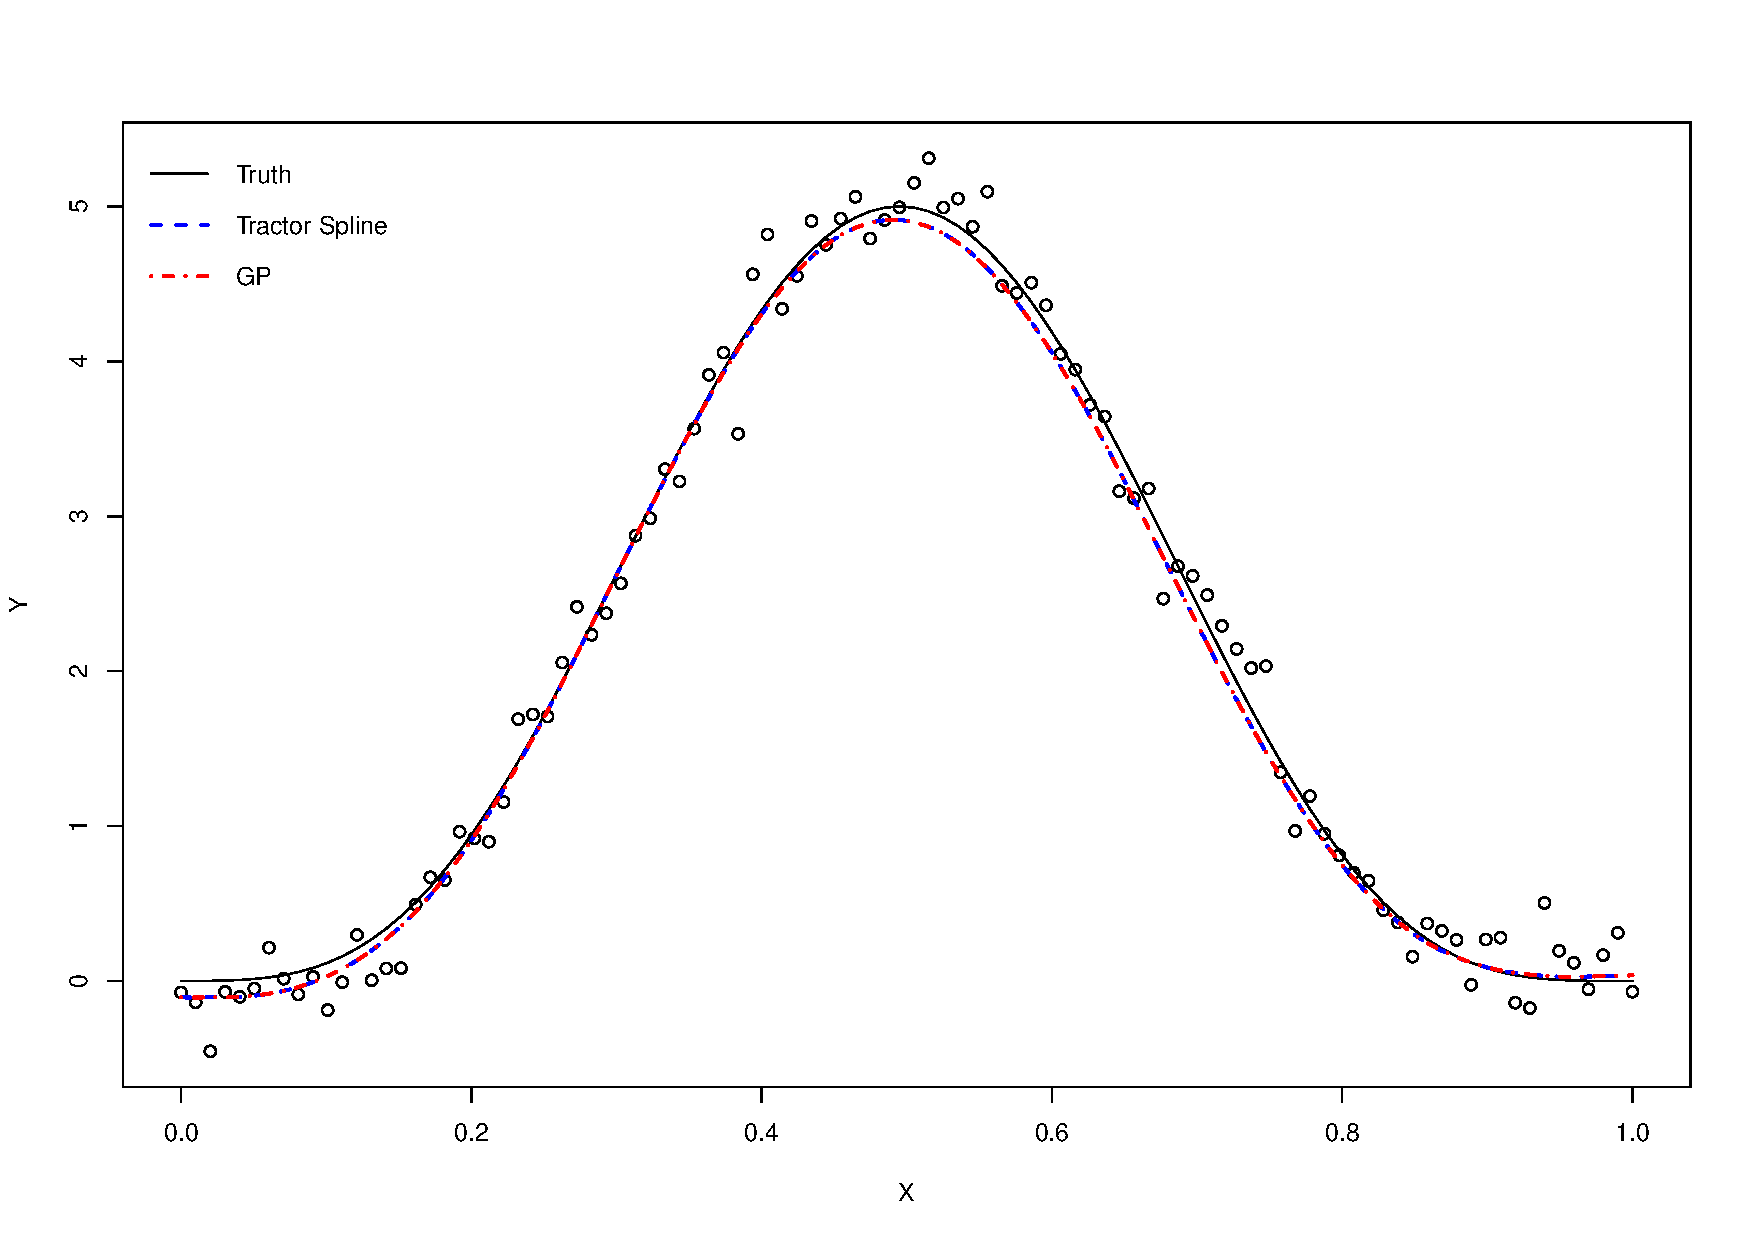
\includegraphics[width=12cm,height=7cm]{Chapters/03GPR/plot/sim_cov} \\
 \caption{Comparing two methods. In this graph, the blue line is reconstruction from tractor spline, the red line is the mean of Gaussian Process, which is the posterior $\mathbb{E}(\eta(x) | \mathbf{Y}, \mathbf{V})$.}
\end{figure}


The leave-one-out cross validation score of a tractor spline is
\begin{equation}
\mbox{LOOCV}(\lambda,\gamma)=\frac{1}{n}\sum_{i=1}^{n}\left( \frac{\hat{f}(t_i)-y_i+\frac{\gamma T_{ii}}{1-\gamma V_{ii}}(\hat{f}'(t_i)-v_i)}{1-S_{ii}-\frac{\gamma T_{ii}}{1-\gamma V_{ii}}U_{ii}} \right)^2.
\end{equation}
Followed by the approximation $S_{ii}\approx\frac{1}{n}\mbox{tr}(S)$, $T_{ii}\approx\frac{1}{n}\mbox{tr}(T)$, $U_{ii}\approx\frac{1}{n}\mbox{tr}(U)$ and $V_{ii}\approx\frac{1}{n}\mbox{tr}(V)$ (Ali R. Syed 2011), the generalized cross validation criterion (GCV) (Wahba, 1990) is
\begin{equation}
\mbox{GCV}(\lambda,\gamma)=\frac{1}{n}\sum_{i=1}^{n}\left( \frac{\hat{f}(t_i)-y_i+ \frac{\gamma\mbox{tr}(T)/n}{1-\gamma \mbox{tr}(V)/n}(\hat{f}'(t_i)-v_i)}{1-\mbox{tr}(S)/n-\frac{\gamma\mbox{tr}(T)/n}{1-\gamma \mbox{tr}(V)/n} \mbox{tr}(U)/n} \right)^2,
\end{equation}
which may provide further computational savings since it requires finding the trace rather than the individual diagonal entries of the hat matrix. It can be written in the form of
\begin{equation}
\mbox{GCV}(\lambda,\gamma)=\frac{(\mathbf{\hat{f}}-\mathbf{y})^\top (\mathbf{\hat{f}}-\mathbf{y})+\frac{2\mbox{tr}(\gamma T)}{\mbox{tr}(I-\gamma V)}(\mathbf{\hat{f}}-\mathbf{y})^\top (\mathbf{\hat{f}}'-\mathbf{v}) + \left( \frac{\mbox{tr}(\gamma T)}{\mbox{tr}(I-\gamma V)} \right)^2 (\mathbf{\hat{f}}'-\mathbf{v})^\top (\mathbf{\hat{f}}'-\mathbf{v})}{\left( \mbox{tr}(I-S-\frac{\mbox{tr}(\gamma T)}{\mbox{tr}(I-\gamma V)}U) \right)^2}.
\end{equation}
A natural extension of the above GCV for tractor spine with correlated errors is
\begin{equation}
\mbox{GCV}(\lambda,\gamma)=\frac{(\mathbf{\hat{f}}-\mathbf{y})^\top W(\mathbf{\hat{f}}-\mathbf{y})+\frac{2\mbox{tr}(\gamma T)}{\mbox{tr}(I-\gamma V)}(\mathbf{\hat{f}}-\mathbf{y})^\top W^{1/2}U^{\top 1/2}(\mathbf{\hat{f}}'-\mathbf{v}) + \left( \frac{\mbox{tr}(\gamma T)}{\mbox{tr}(I-\gamma V)} \right)^2 (\mathbf{\hat{f}}'-\mathbf{v})^\top U(\mathbf{\hat{f}}'-\mathbf{v})}{\left( \mbox{tr}(I-S-\frac{\mbox{tr}(\gamma T)}{\mbox{tr}(I-\gamma V)}U) \right)^2}.
\end{equation}




\section{Numeric Simulation of Smoothing Spline and GPR}
Given $\mathbf{X}$ a length-10 sequence from 0 to 1, 
\begin{align*}
\mathbf{Y}&=\left[1,3,4,7,10,18,25,39,48,59 \right],
\end{align*}
$v_i=\begin{cases}
\frac{y_{i+1}-y_i}{x_{i+1}-x_i}&\mbox{if } 1\leq i \leq 9\\
0 & \mbox{if } i=10
\end{cases}$. 
A simulated result is in figure 1.
\begin{figure}[h]  
	\centering
	\begin{tabular}{c}
		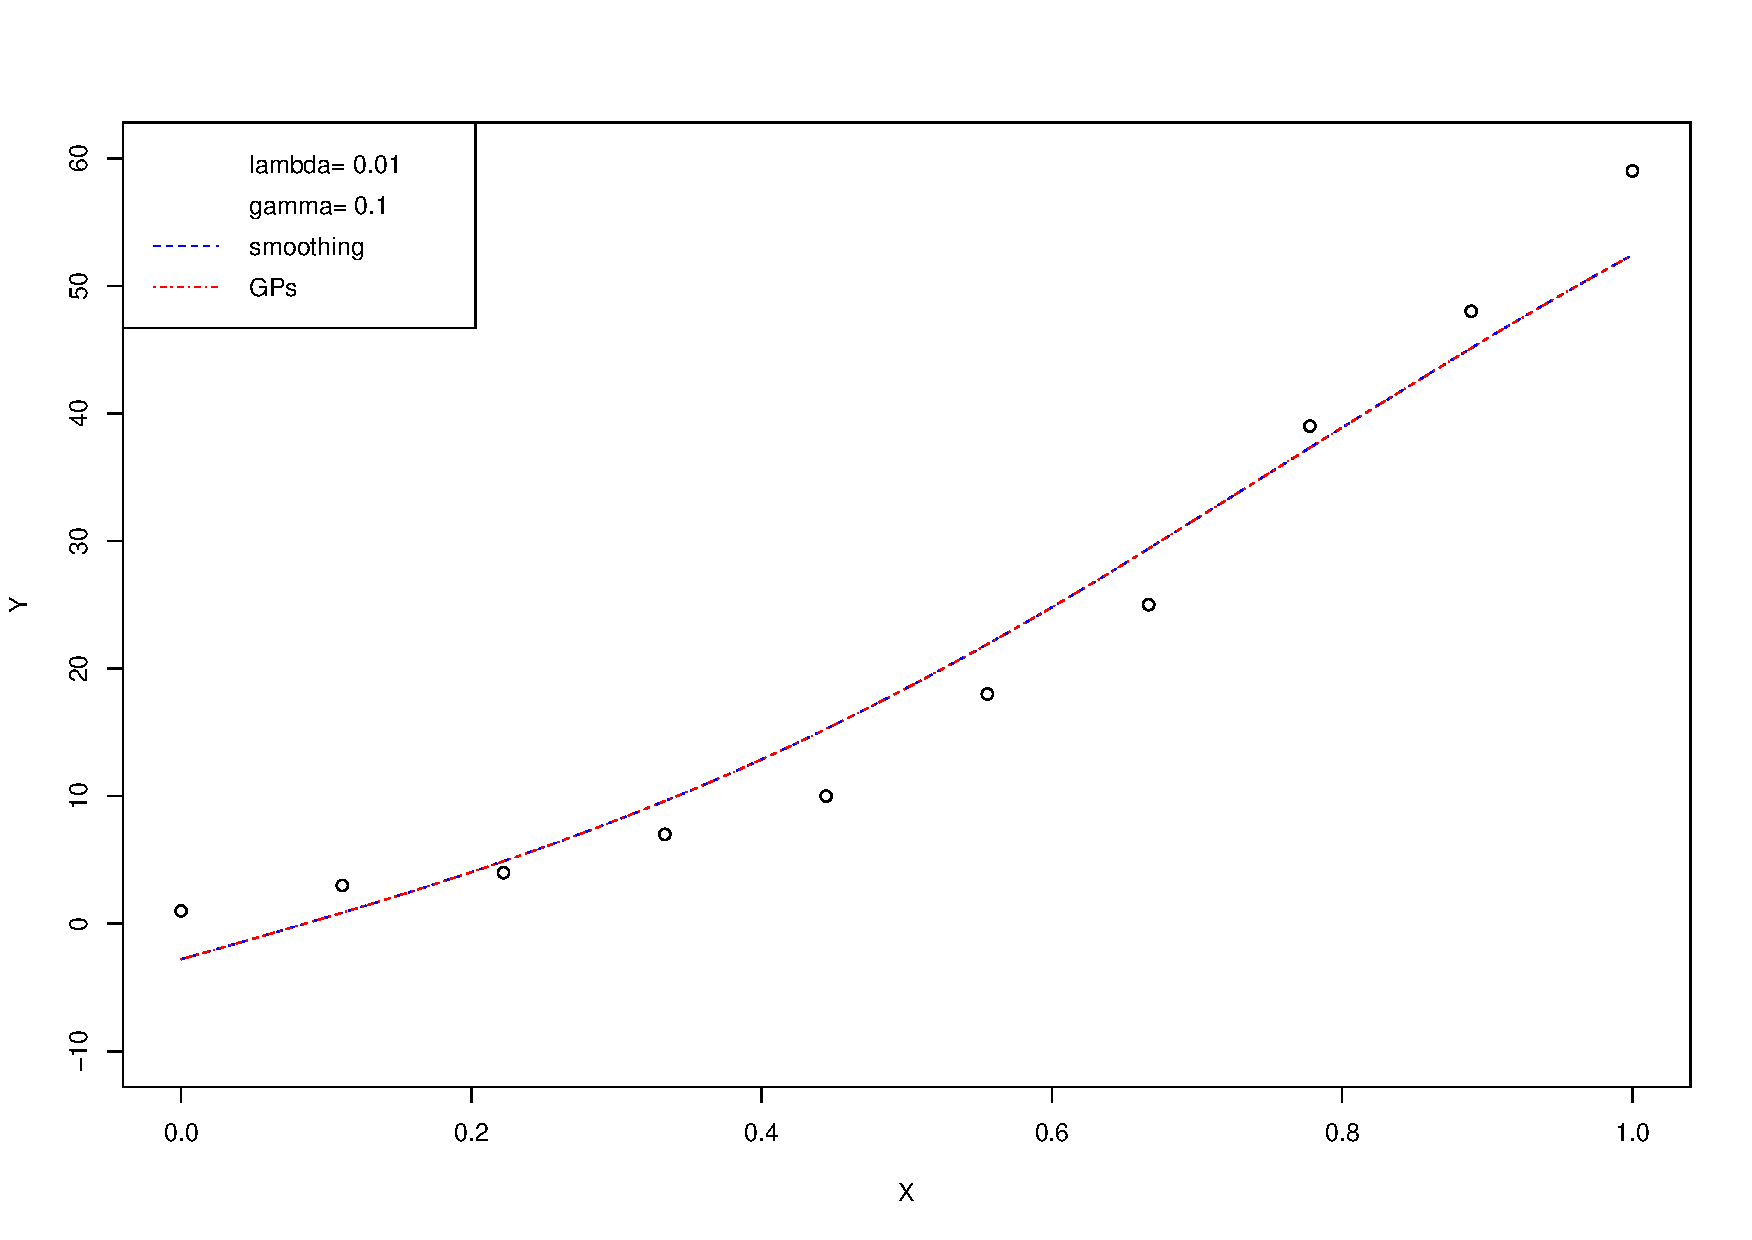
\includegraphics[width=12cm,height=7cm]{Chapters/03GPR/plot/simu01} \\[\abovecaptionskip]
		\small (a) 
	\end{tabular}
	%    \vspace{\floatsep}
	\begin{tabular}{c}
		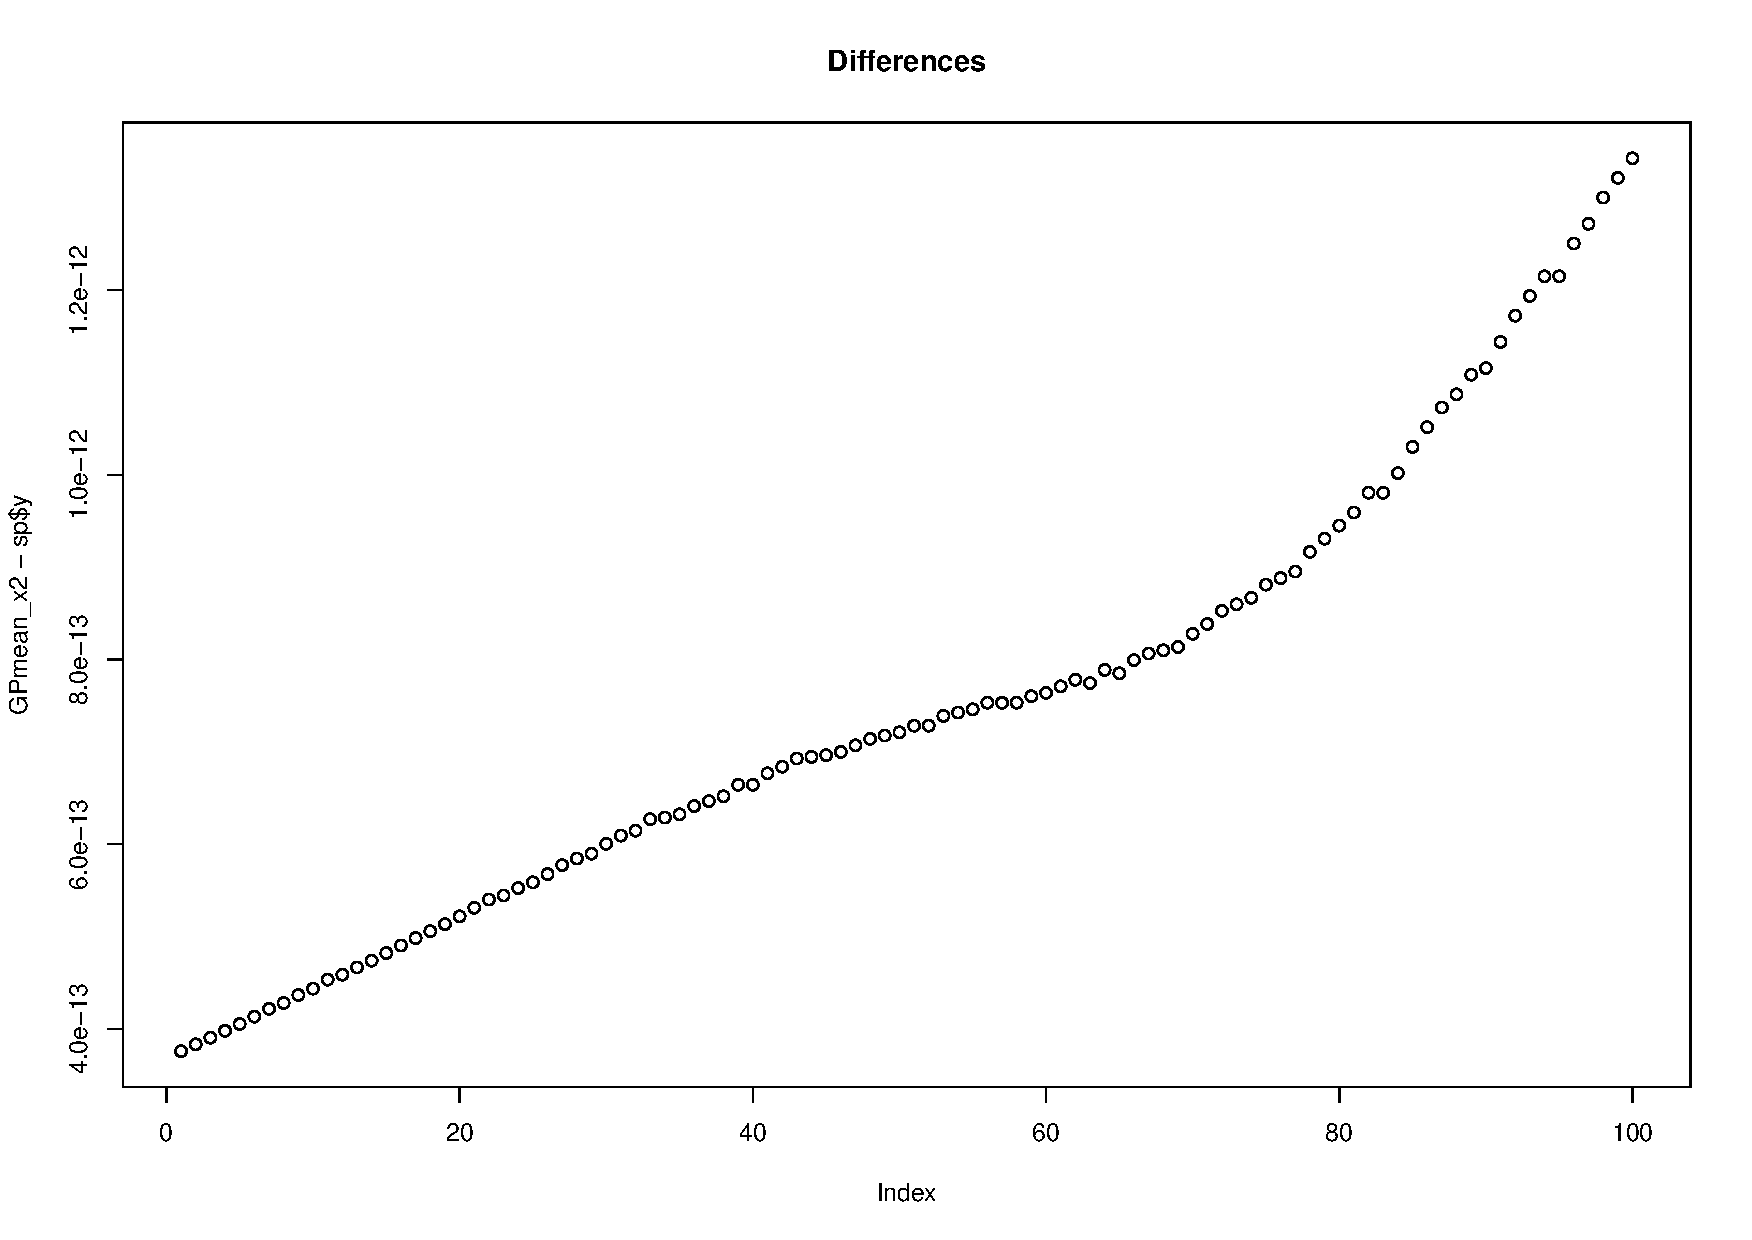
\includegraphics[width=12cm,height=7cm]{Chapters/03GPR/plot/simu02} \\[\abovecaptionskip]
		\small (b) 
	\end{tabular}
	\caption{(a) Comparing two methods under the same parameters $\lambda=0.01$ and $\gamma=0.1$. In this graph, the blue line is reconstruction from tractor spline, the red line is the mean of Gaussian Process, which is the posterior $\E (f(x) \mid  \mathbf{Y}, \mathbf{V})$. (b) The differences between two methods under the same parameters.}
\end{figure}



